\chapter{Neutrino physics}\label{chapter:neutrinos}

\begin{chapquote}{Terry Pratchett, \textit{Sourcery}}
	Little particles of inspiration sleet through the universe all the time traveling through the densest matter in the same way that a neutrino passes through a candyfloss haystack, and most of them miss.
\end{chapquote}

%\noindent
Ever since they were postulated in 1930 by Wolfgang Pauli to explain the continuous $\beta$ decay spectrum \cite{Pauli1930}, and later found by F. Reines and C. Cowan at the Savannah River reactor in 1953 \cite{Reines1953}, neutrinos have had a special place among all other elementary particles. They provide a unique way to probe a wide range of physics, from nuclear physics to cosmology, from astrophysics to colliders. Moreover, there is compelling evidence to believe that the study of neutrinos may be the key to unveiling different aspects of \gls{bsm} physics, difficult to test elsewhere \cite{Arguelles2019}.

In this Chapter, I review the basics of neutrino physics, from their role within the \gls{sm} to the main open questions related to the neutrino sector, paying special attention to the phenomenology of neutrino oscillations.

\section{Neutrinos in the SM}\label{sec:sm_and_nu}

The \gls{sm} of fundamental interactions was initially proposed in 1967 by S. Glashow, S. Weinberg and A. Salam\cite{Glashow1961,Weinberg1967,Salam1968}. This theoretical framework describes the dynamics of leptons and quarks, by introducing a collection of mediating gauge vector bosons and one scalar particle, known as the Higgs boson. It assumes that the local gauge symmetry ${\mathrm{SU}(3)\times\mathrm{SU}(2)_{\mathrm{L}}\times\mathrm{U}(1)_{\mathrm{Y}}}$ is an internal symmetry of the system, with $\mathrm{SU}(3)$ describing quantum chromodynamics, and ${\mathrm{SU}(2)_{\mathrm{L}}\times\mathrm{U}(1)_{\mathrm{Y}}}$ being the gauge groups of the electroweak sector. For a detailed overview of the \gls{sm} of electroweak interactions, see Ref. \cite{Pich2012}.

In the \gls{sm}, neutrinos appear in three flavours, namely $\nu_{e}$, $\nu_{\mu}$, and $\nu_{\tau}$. These are associated with the corresponding charged leptons, $e$, $\mu$, and $\tau$. Neutrinos exist only as left-handed particles, grouped in doublets with the charged leptons, while the latter come in both chirality states:
\begin{equation}
	\begin{array}{cccccc}
		\begin{pmatrix}\nu_{e}\\e^{-}_{L}\end{pmatrix},&\begin{pmatrix}\nu_{\mu}\\\mu^{-}_{L}\end{pmatrix},&\begin{pmatrix}\nu_{\tau}\\\tau^{-}_{L}\end{pmatrix},&e^{-}_{R},&\mu^{-}_{R},&\tau^{-}_{R}.
	\end{array}
\end{equation}
Similarly, quarks also exist in both chirality states, and are grouped as:
\begin{equation}
	\begin{array}{ccccccccc}
		\begin{pmatrix}u_{L}\\d_{L}\end{pmatrix},&\begin{pmatrix}s_{L}\\c_{L}\end{pmatrix},&\begin{pmatrix}t_{L}\\b_{L}\end{pmatrix},&u_{R},&d_{R},&s_{R},&c_{R},&t_{R},&b_{R}.
	\end{array}
\end{equation}

The absence of right-handed neutrino fields implies that neutrinos are strictly massless within the \gls{sm}. This restriction follows from the experimental observation that all neutrinos produced via weak interactions are pure left-handed helicity states \cite{Goldhaber1958} (and similarly antineutrinos are pure right-handed states). The hypothetical existence of right-handed neutrinos could be indirectly inferred from the observation of non-zero neutrino masses. Nevertheless, the existence of neutrino masses is not a sufficient condition for the existence of such fields.

Left and right-handed fermions transform differently under $\mathrm{SU}(2)_{\mathrm{L}}\times\mathrm{U}(1)_{\mathrm{Y}}$ rotations, as the right-handed particles are singlets under $\mathrm{SU}(2)_{\mathrm{L}}$. Applying a local transformation, they change as:
\begin{equation}
	\begin{split}
		\psi_{L} &\longrightarrow \mathrm{e}^{-iY\beta(x)/2}~\mathrm{e}^{-iT_{a}\alpha_{a}(x)}~\psi_{L},\\
		\psi_{R} &\longrightarrow \mathrm{e}^{-iY\beta(x)/2}~\psi_{R},
	\end{split}
\end{equation}
where $Y/2$ and $T_{a}$ are the generators of $\mathrm{U}(1)_{\mathrm{Y}}$ and $\mathrm{SU}(2)_{\mathrm{L}}$, respectively, and $\beta(x)$ and $\alpha_{a}(x)$ are the parameters of the rotation.

The values of the quantum numbers $Y/2$ and $T_{3}$, the weak hypercharge and the third component of the weak isospin, have to be assigned to the different particles. The values of $T_{3}$ follow from the assigned $\mathrm{SU}(2)$ representations of the matter fields. After the spontaneous symmetry breaking $\mathrm{SU}(2)_{\mathrm{L}}\times\mathrm{U}(1)_{\mathrm{Y}} \rightarrow \mathrm{U}(1)_{\mathrm{EM}}$, one finds the relation which determines the electric charge:
\begin{equation}
	Q = T_{3} + \frac{Y}{2}.
\end{equation}
Setting the electric charge to $-1$ for electrons, we can find the values of the weak hypercharge for the rest of the fermions. The resulting values for the first generation of leptons and quarks are shown in Tab. \ref{tab:sm_charge}.

\begin{table}[t]
	\centering
	\caption{Values of $T_{3}$ and $Y/2$ assigned to the first generation of fermions.}
		\begin{tabular}{l|ccccccc}
			& $e_{L}$ & $\nu_{e}$ & $e_{R}$ & $u_{L}$ & $d_{L}$ & $u_{R}$ & $d_{R}$ \\[2mm] \hline
			\rule{0pt}{1.1\normalbaselineskip}$T_{3}$ & $-1/2$  & $1/2$     & $0$     & $1/2$   & $-1/2$  & $0$     & $0$     \\[2mm]
			$Y/2$   & $-1/2$  & $-1/2$    & $-1$    & $1/6$   & $1/6$   & $2/3$   & $-1/3$ 
		\end{tabular}
	\label{tab:sm_charge}
\end{table}

It is clear that the free Lagrangian of the theory is not invariant under the gauge transformations, as the kinetic terms contain derivatives. Therefore, to make it invariant one needs to introduce a set of gauge bosons. They appear in the so-called covariant derivative, which replaces the common derivative and transforms in the same way as the fermion fields under local rotations. This constraint fixes completely the transformations of the spin-1 fields. For left and right-handed particles, the covariant derivatives are given by:
\begin{equation}
	\begin{split}
		D_{\mu} \psi_{L} &= \left(\partial_{\mu} + ig'\frac{Y}{2}B_{\mu}+igT_{a}W^{a}_{\mu}\right)\psi_{L},\\
		D_{\mu} \psi_{R} &= \left(\partial_{\mu} + ig'\frac{Y}{2}B_{\mu}\right)\psi_{R},
	\end{split}
\end{equation}
where $W^{i}_{\mu}$, $i=1,2,3$ and $B_{\mu}$ are the gauge bosons for the $\mathrm{SU}(2)_{\mathrm{L}}$ and $\mathrm{U}(1)_{\mathrm{Y}}$ groups, respectively, and $g$ and $g'$ are the corresponding gauge couplings. It can be shown that these fields transform in the adjoint representation of the gauge group.

So far, the theory only contains massless particles, as adding bare mass terms to the Lagrangian would spoil the gauge symmetry. Therefore, the mass terms need to be induced by a spontaneous breaking of the symmetries. In the \gls{sm}, this is achieved by the Higgs mechanism \cite{Englert1964,Higgs1964,Guralnik1964}. The Higgs doublet is coupled to the gauge bosons through the covariant derivative, and to the fermions through the Yukawa couplings \cite{Pich2012}. Upon spontaneous symmetry breaking, the vacuum expectation value of the Higgs field generates the mass terms of the particles.

\begin{table}[t]
	\centering
	\caption{Neutral current couplings.}
			\begin{tabular}{l|cccc}
					& $u$                                       & $d$                                        & $\nu_{e}$ & $e$                              \\[2mm] \hline
			\rule{0pt}{1.1\normalbaselineskip}$2v_{f}$ & $1-\frac{8}{3}\mathrm{sin}^{2}\theta_{W}$ & $-1+\frac{4}{3}\mathrm{sin}^{2}\theta_{W}$ & $1$       & $-1+4\mathrm{sin}^{2}\theta_{W}$ \\[2mm]
			$2a_{f}$ & $1$                                       & $-1$                                       & $1$       & $-1$                            
		\end{tabular}
	\label{tab:sm_nc_couplings}
\end{table}

In order to obtain the physical intermediate vector boson states, we need to perform the following redefinitions:
\begin{equation}
	\begin{split}
		A_{\mu} &= \mathrm{sin}~\theta_{W} W^{3}_{\mu} + \mathrm{cos}~\theta_{W} B_{\mu},\\
		Z_{\mu} &= \mathrm{cos}~\theta_{W} W^{3}_{\mu} - \mathrm{sin}~\theta_{W} B_{\mu},\\
		W^{\pm}_{\mu} &= \frac{1}{\sqrt{2}}\left(W^{1}_{\mu} \mp i W^{2}_{\mu}\right),
	\end{split}
\end{equation}
where $A_{\mu}$ is the photon field, and $Z_{\mu}$ and $W^{\pm}_{\mu}$ are the neutral and the charged weak boson fields, respectively. The Weinberg angle, $\theta_{W}$, can be written in terms of the gauge couplings:
\begin{equation}
	\begin{split}
		\mathrm{cos}~\theta_{W} &= \frac{g}{\sqrt{g^{2}+{g'}^{2}}},\\
		\mathrm{sin}~\theta_{W} &= \frac{g'}{\sqrt{g^{2}+{g'}^{2}}}.
	\end{split}
\end{equation}
The gauge couplings and the Weinberg angle allow to express the electric charge as $e = g'~\mathrm{cos}~\theta_{W} = g~\mathrm{sin}~\theta_{W}$.

At this point, the interacting part of the electroweak Lagrangian can be re-written as the sum of three contributions: the electromagnetic (EM), charged-current (\gls{cc}) and neutral-current (\gls{nc}) components:
\begin{equation}\label{eq:int_lagrangian}
	\begin{split}
		\mathcal{L}^{int}_{\mathrm{EW}} &= \mathcal{L}_{\mathrm{EM}}+\mathcal{L}_{\mathrm{CC}}+\mathcal{L}_{\mathrm{NC}}\\
		&= -e A_{\mu} J^{\mu}_{\mathrm{EM}} - \frac{g}{2\sqrt{2}} \left(W^{+}_{\mu}J^{\mu}_{\mathrm{CC}} + \mathrm{h.c.}\right) - \frac{g}{2 \mathrm{cos}\theta_{W}} Z_{\mu} J^{\mu}_{\mathrm{NC}},
	\end{split}
\end{equation}
with $+ \mathrm{h.c.}$ being an abbreviation for adding the Hermitian conjugate of the preceding terms and the currents defined as:
\begin{equation}\label{eq:currents}
	\begin{split}
		J^{\mu}_{\mathrm{EM}} &= \sum_{f} Q_{f} \bar{f}\gamma^{\mu}f,\\
		J^{\mu}_{\mathrm{CC}} &= \sum_{\ell}\bar{\nu}_{\ell}\gamma^{\mu}(1-\gamma_{5})\ell + \sum_{f}\bar{u}_{f}\gamma^{\mu}(1-\gamma_{5})d_{f},\\
		J^{\mu}_{\mathrm{NC}} &= \sum_{f} \bar{f}\gamma^{\mu}(v_{f} - a_{f}\gamma_{5})f,\\
	\end{split}
\end{equation}
where $f$ denotes any \gls{sm} fermion, $\ell$ and $\nu_{\ell}$ a charged lepton and a neutrino of any flavour, and $u_{f}$ and $d_{f}$ an up-like and a down-like quark of any flavour\footnote{Note that these fields are written in the flavour basis. Moving to the mass eigenstates one has to introduce the \gls{ckm} matrix, which induces transitions between up- and down-like quarks from different generations.}. For the \gls{nc} case, the values of the $v_{f}$ and $a_{f}$ couplings are given in Tab. \ref{tab:sm_nc_couplings}.

As seen in Eqs. (\ref{eq:int_lagrangian}) and (\ref{eq:currents}), in the electroweak theory neutrinos are coupled to the $Z$ boson in a flavour universal way. Therefore, by measuring the so-called invisible decay width of the $Z$ boson we have an estimate of the number of light (i.e. lighter than the $Z$ boson) neutrino flavours. This number was measured by \gls{lep} in a combined analysis of $e^{+}e^{-} \rightarrow \mu^{+}\mu^{-}$ and $e^{+}e^{-} \rightarrow \mathrm{hadrons}$ to be $N_{\nu} = 2.9840 \pm 0.0082$ \cite{ALEPH2005}.

\section{Trouble in the neutrino sector}\label{sec:nu_trouble}

\subsection{The solar neutrino problem}

Neutrinos are produced everywhere in vast amounts. One of the most prominent sources of neutrinos in our vicinity is our Sun. The Sun is powered mainly by two nuclear fusion reactions, the $\mathrm{p}-\mathrm{p}$ chain and the CNO cycle \cite{Adelberger2010}. In both cases, the overall reaction is:
\begin{equation}
	4~\prescript{1}{}{\mathrm{H}}^{+}+2~e^{-} \longrightarrow \prescript{4}{}{\mathrm{He}}^{2+} + 2~\nu_{e} + 26.73~\mathrm{MeV},
\end{equation}
where hydrogen is converted to helium and part of the released energy is lost to the neutrinos. The electron neutrinos produced are often labelled after the processes that generate them. Figure \ref{fig:solar_nu_flux} shows the solar neutrino flux as a function of the neutrino energy, broken down by the production process.

In the late 1960s, the Brookhaven Solar Neutrino Experiment, led by R. Davis, started data taking with the goal of measuring the solar neutrino flux \cite{Davis1968}. The experiment used a tank containing $380~\mathrm{m}^{3}$ of tetrachloroethene ($\mathrm{C}_{2}\mathrm{Cl}_{4}$), a liquid commonly used in dry-cleaning, located $1.5~\mathrm{km}$ underground in the Homestake mine in Lead, South Dakota. The incoming neutrinos would get captured following the reaction:
\begin{equation}
	\nu_{e} + \prescript{37}{}{\mathrm{Cl}} \longrightarrow \prescript{37}{}{\mathrm{Ar}}^{+} + e^{-},
\end{equation}
allowing a measurement of the neutrino flux by counting the $\prescript{37}{}{\mathrm{Ar}}$ isotopes. The threshold for this reaction is $0.814~\mathrm{MeV}$, just below the $0.862~\mathrm{MeV}$ line from the $\prescript{7}{}{\mathrm{Be}}$ ground state transition.

\begin{figure}[t]
	\centering
	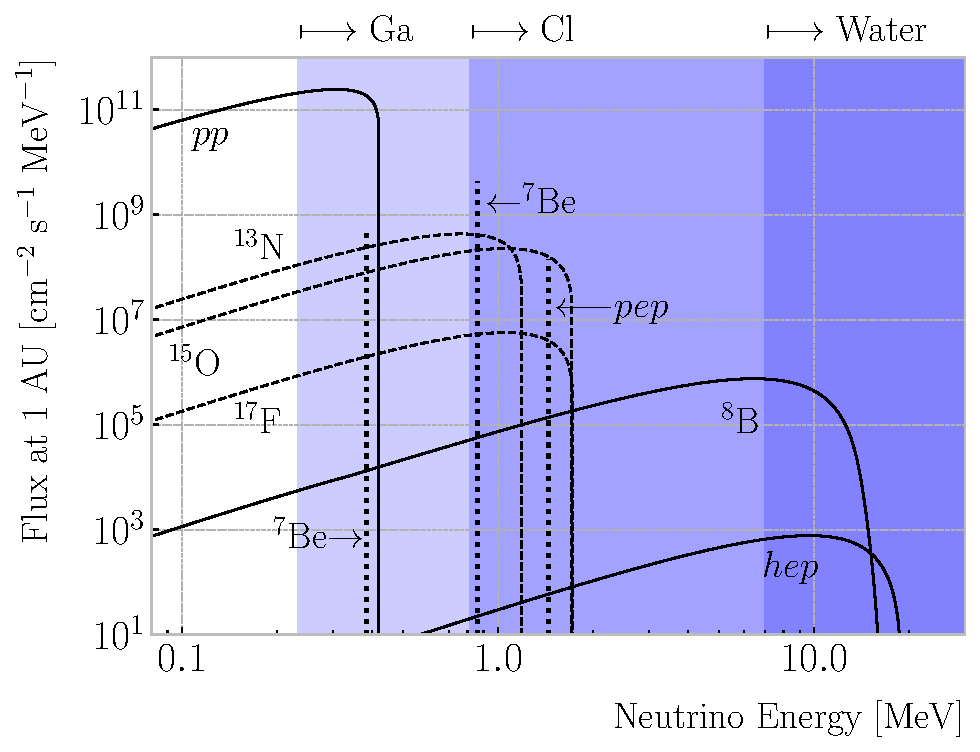
\includegraphics[width=.75\linewidth]{Images/Nu/solar_neutrino_flux.pdf}
	\caption[Solar neutrino fluxes for the solar model BS05(OP).]{Solar neutrino fluxes for the solar model BS05(OP). The detection thresholds for Gallium, Chlorine and water-based experiments are also shown. Figure adapted from Ref. \cite{Bahcall2004}.}
	\label{fig:solar_nu_flux}
\end{figure}

The results of the experiment were compared to the theoretical predictions made by J. Bahcall \cite{Bahcall1968}. During its operation from 1968 to 2002, the experiment observed a solar $\nu_{e}$ flux that was approximately a third of the total prediction \cite{Cleveland1998}.

In the early 1990s, the \gls{sage} \cite{SAGE2009} and \gls{gallex} \cite{GALLEX2010} experiments started operations. The detection principle used for both experiments was similar to that of the Homestake experiment, but using $\prescript{71}{}{\mathrm{Ga}}$ instead of $\mathrm{C}_{2}\mathrm{Cl}_{4}$. With a detection threshold of $0.233~\mathrm{MeV}$, the Gallium-based experiments were able to observe the $pp$ neutrino flux. Both experiments measured a solar electron neutrino flux that was a factor of two lower than the predictions, demonstrating that this deficit was energy-dependent.

In the early 2000s, the \gls{sno} experiment put an end to the solar neutrino puzzle \cite{Ahmad2001,Ahmad2002}. Thanks to its directional capabilities, being a Cherenkov light detector, as well as to its heavy water target, \gls{sno} measured the total solar neutrino flux through the \gls{nc} process:
\begin{equation}
	\nu_{\alpha} + d \longrightarrow n + p + \nu_{\alpha},
\end{equation}
where $d$ denotes the deuterium nucleus and $\alpha = e, \mu, \tau$. This measurement agreed with the solar model predictions. Then, measuring the \gls{cc} reaction:
\begin{equation}
	\nu_{e} + d \longrightarrow p + p + e^{-},
\end{equation}
they were able to establish that the $\nu_{\mu}$ and $\nu_{\tau}$ solar fluxes are in fact non-zero, revealing that electron neutrinos were transitioning into different flavours.

\subsection{The atmospheric neutrino problem}

When cosmic-rays interact with the atoms in the upper atmosphere, a plethora of hadrons, mainly $\pi$ and $K$ mesons, are produced. In particular, for the charged pions, the following decay chain dominates:
\begin{equation}
	\begin{split}
		&\pi^{+} \longrightarrow \mu^{+} + \nu_{\mu},\\
		&\mu^{+} \longrightarrow e^{+} + \bar{\nu}_{\mu} + \nu_{e},
	\end{split}
\end{equation}
and similar for the antiparticles, as the relevant matrix elements for the meson decays are proportional to the lepton mass. For neutrino energies $< 1~\mathrm{GeV}$, the ratio:
\begin{equation}
	\frac{N(\nu_{\mu}+\bar{\nu}_{\mu})}{N(\nu_{e}+\bar{\nu}_{e})},
\end{equation}
of produced neutrinos and antineutrinos is, to a good approximation, equal to two \cite{Gaisser2002}.

During the 1980s, several proton decay experiments, like Kamiokande \cite{Hirata1988}, \gls{imb} \cite{Casper1991}, \gls{macro} \cite{Ambrosio1998}, and Soudan-2 \cite{Allison1997}, measured the flux of atmospheric neutrinos. This was an important part of their research programme, as the atmospheric neutrinos constitute their main background. All these experiments reported an atmospheric neutrino ratio lower than the predictions.

\begin{figure}[t]
	\centering
	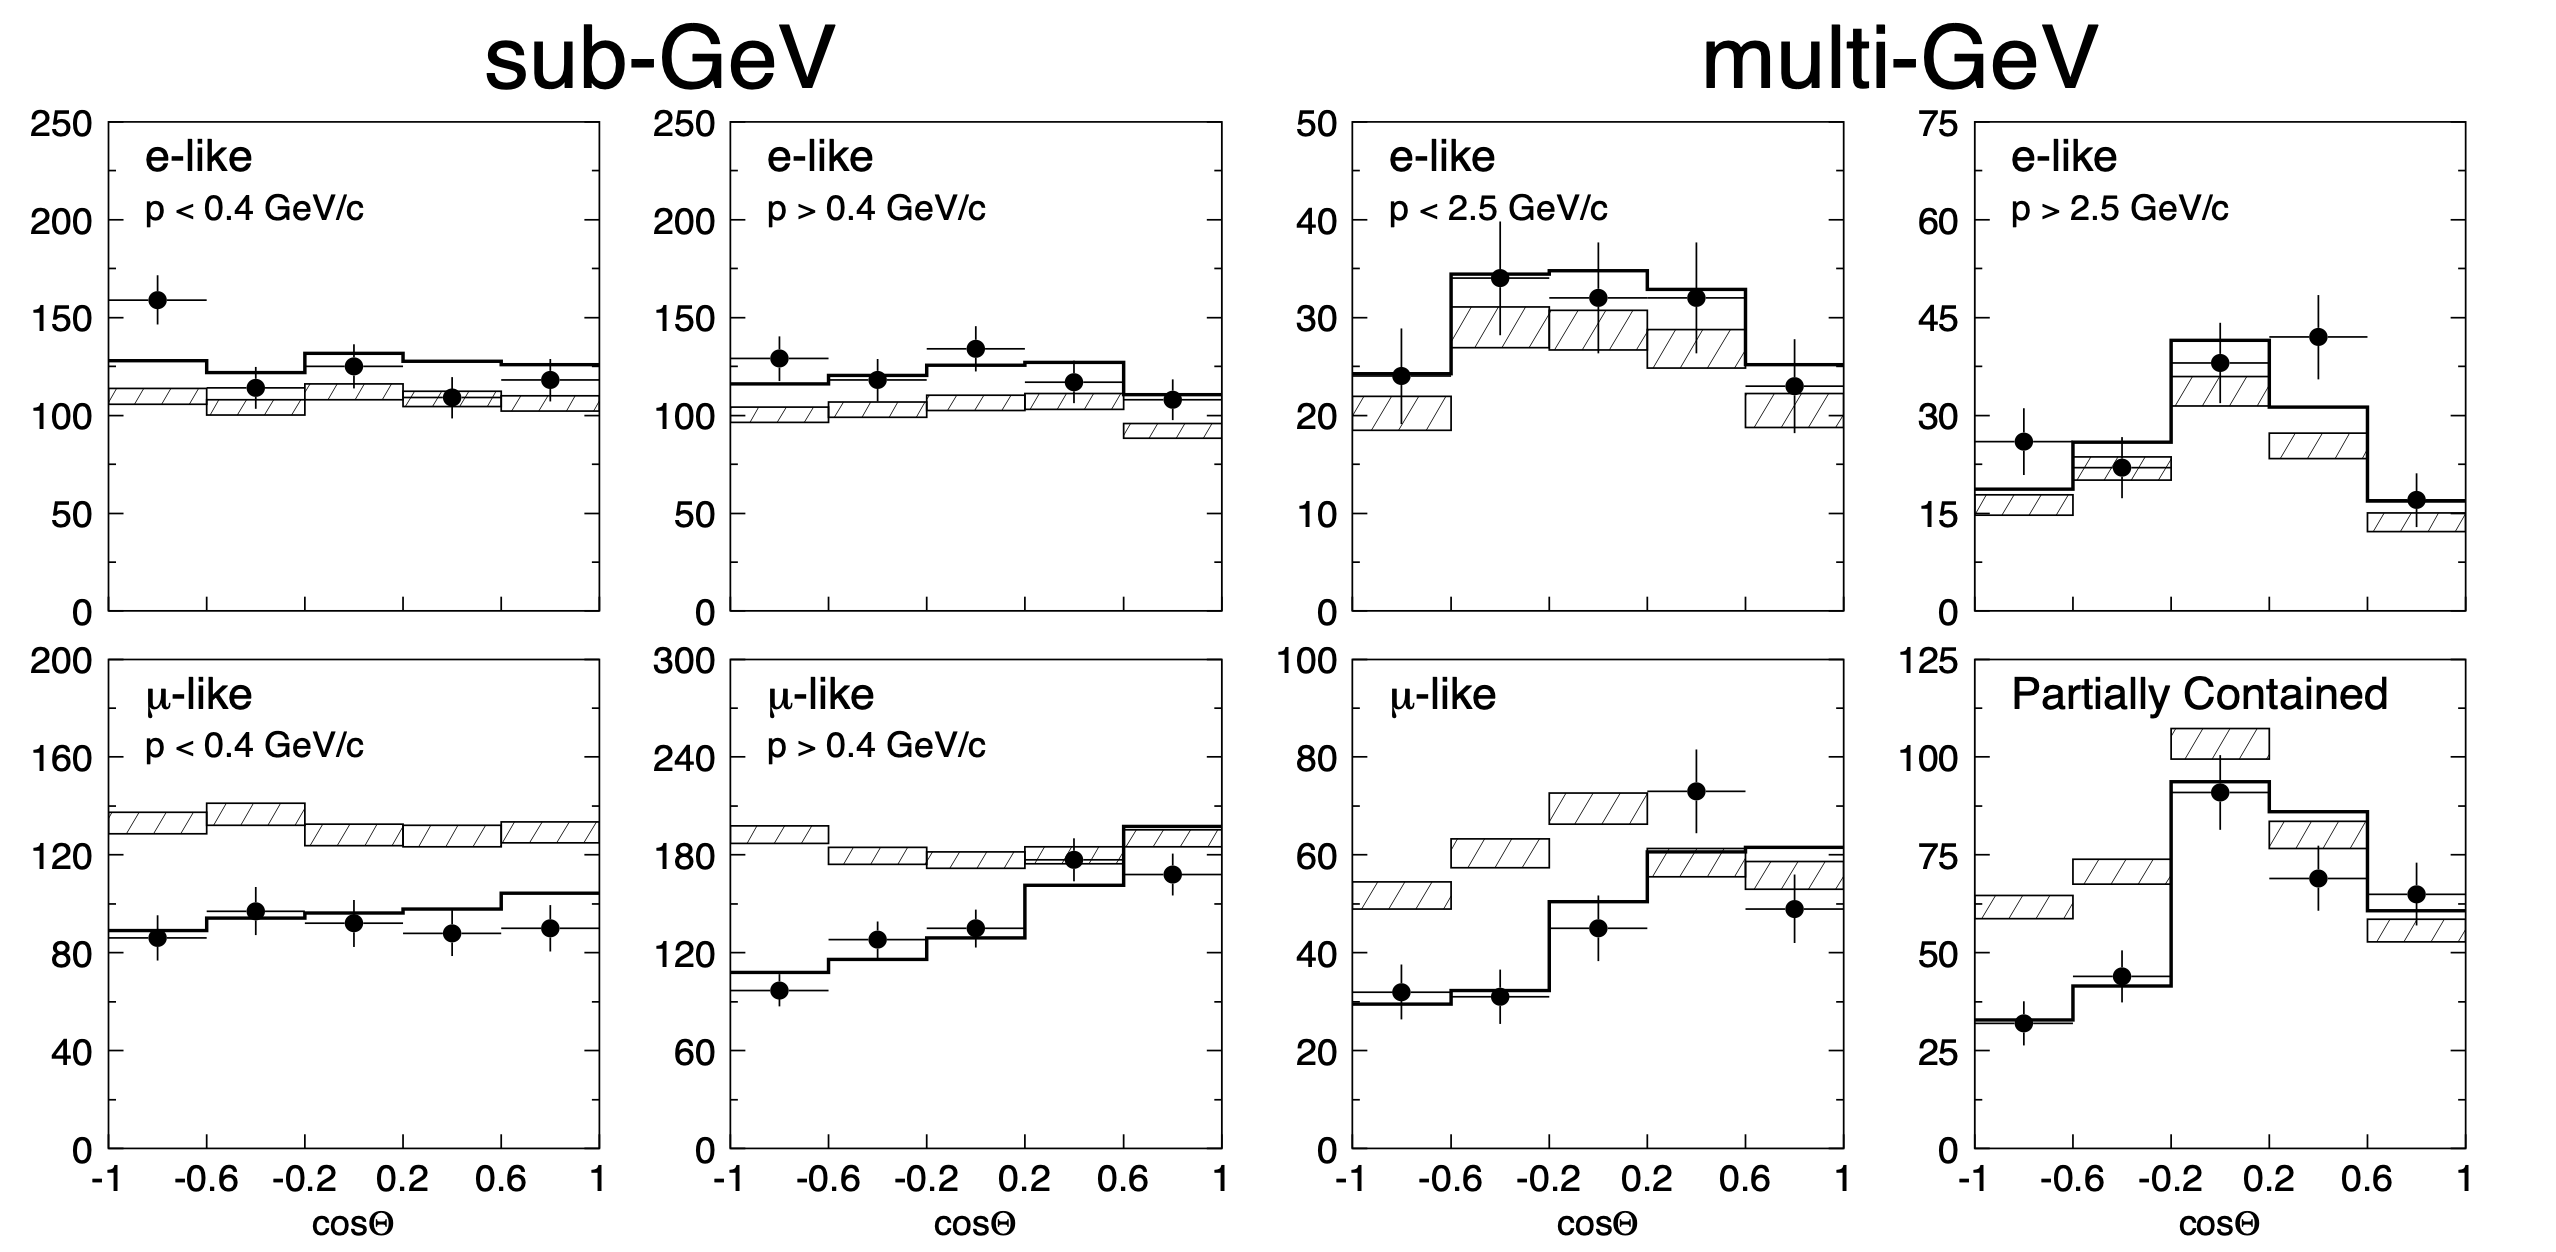
\includegraphics[width=.90\linewidth]{Images/Nu/superk_oscillations.png}
	\caption[Zenith angle distributions for the selected $\nu_{e}$ and $\nu_{\mu}$ events in the \gls{sk} detector.]{Zenith angle distributions for the selected $\nu_{e}$ (top row) and $\nu_{\mu}$ (bottom row) events in the \gls{sk} detector. The hatched region corresponds to the expectation in the case of no oscillations, whereas the solid line indicates the best-fit in the case of $\nu_{\mu} \rightarrow \nu_{\tau}$ oscillations. Figure taken from Ref. \cite{SuperKamiokande1998}.}
	\label{fig:atmospheric_nu_osc}
\end{figure}

A few years before the \gls{sno} discovery, in 1998, the Super-Kamiokande collaboration (\gls{sk}) measured the atmospheric $\nu_{e}$ and $\nu_{\mu}$ spectra as a function of the zenith angle \cite{SuperKamiokande1998}. Upward-going particles have negative zenith angle, $\mathrm{cos}~\Theta < 0$, indicating that they entered from the bottom of the detector. These upward-going neutrinos had to travel through the Earth in order to reach the detector, allowing \gls{sk} to probe a broad range of baselines. Figure \ref{fig:atmospheric_nu_osc} shows the reported distributions (black dots), compared to the no oscillations prediction (hatched region). This measurement confirmed that muon neutrinos transition to other flavours, and that this phenomenon depends both on the energy and the path length of the neutrino.

The \gls{sk} and \gls{sno} findings provided definitive evidence for the existence of neutrino oscillations, and therefore non-zero neutrino masses. This constitutes one of the groundbreaking discoveries of modern physics and has acted as driving force for \gls{bsm} searches. The minimal extension of the \gls{sm} we can make to address this phenomenon is introducing different masses for at least two of the neutrinos. This way, we are left with three neutrino mass eigenstates $\nu_{1}$, $\nu_{2}$, and $\nu_{3}$, with masses $m_{1}$, $m_{2}$, and $m_{3}$ respectively, which in general will not coincide with the flavour eigenstates, $\nu_{e}$, $\nu_{\mu}$, and $\nu_{\tau}$.

\section{Massive neutrinos}\label{sec:nu_mass}

The existence of neutrino oscillations imply that neutrinos are massive particles. However, as we have seen before, within the \gls{sm} neutrinos are massless, as they do not have a mass term in the Lagrangian. If one wants to give neutrinos a mass, the particle content of the \gls{sm} needs to be expanded.

A way of generating massive neutrinos while maintaining gauge invariance is by introducing an arbitrary number of sterile neutrinos $N_{i}$, $i=1,\dots,m$. These allow for two different types of neutrino mass terms \cite{Gonzalez-Garcia2007}:
\begin{equation}\label{eq:nu_mass_lagrangian}
	-\mathcal{L}_{M_{\nu}} = \sum_{i=1}^{m} \sum_{j=1}^{3} M^{ij}_{D} \bar{N}_{i} \nu_{Lj} + \frac{1}{2} \sum_{i=1}^{m} \sum_{j=1}^{m} M^{ij}_{N} \bar{N}_{i} N^{c}_{j} + \mathrm{h.c.},
\end{equation}
where $M_{D}$ is a complex $m \times 3$ matrix and $M_{N}$ a complex and symmetric $m \times m$ matrix. The first term, often referred to as the Dirac mass term, arises from the corresponding Yukawa interaction after the spontaneous electroweak symmetry breaking, similar to the other fermions. The second term, called the Majorana mass term, is allowed in the Lagrangian as it is a singlet of the gauge group. However, it violates lepton number conservation by two units.

If one imposes lepton number symmetry conservation, the Majorana term must vanish, $M_{N}=0$. In this case, if $m=3$ we can identify the sterile neutrinos as the right-handed component of the neutrino field. The Dirac mass matrix can be diagonalised using two unitary matrices, $V^{\nu}_{R}$ and $V^{\nu}_{L}$, as:
\begin{equation}
	M_{D} = V^{\nu}_{R}~\mathrm{diag}(m_{1}, m_{2}, m_{3})~V^{\nu \dagger}_{L},
\end{equation}
where $m_{i}$, $i=1,2,3$ are the masses of the three neutrino mass eigenstates.

The neutrino mass term can be written in terms of the resulting eigenstates as:
\begin{equation}
	-\mathcal{L}_{M_{\nu}} = \sum_{i=1}^{3} m_{i}~\bar{\nu}_{Di} \nu_{Di},
\end{equation}
with:
\begin{equation}
	\nu_{Di} = \left(V^{\nu \dagger}_{L}~\nu_{L}\right)_{i} + \left(V^{\nu \dagger}_{R}~N\right)_{i}.
\end{equation}

In this scenario, both the low energy particle budget and the symmetries of the \gls{sm} have to be modified. Moreover, the masses of the neutrinos are generated exclusively through the Higgs mechanism, which does not explain why they are much smaller than those of the charged leptons.

Going back to the general case, we can re-write Eq. (\ref{eq:nu_mass_lagrangian}) in matrix form as:
\begin{equation}
	-\mathcal{L}_{M_{\nu}} = \frac{1}{2} \begin{pmatrix}\bar{\nu}^{c}_{L},&\bar{N}\end{pmatrix} \begin{pmatrix}0 & M_{D}^{T}\\M_{D} & M_{N}\end{pmatrix}\begin{pmatrix}\nu_{L}\\N^{c}\end{pmatrix} + \mathrm{h.c.} = \bar{\nu}^{c} M_{\nu} \nu + \mathrm{h.c.},
\end{equation}
with $\nu=\begin{pmatrix}\nu_{L}, & N^{c}\end{pmatrix}^{T}$ being a $(3+m)$-dimensional vector grouping the active and the sterile neutrinos. The matrix $M_{\nu}$, which is a complex $(3+m)\times(3+m)$ symmetric matrix, can be diagonalised by means of a unitary matrix $V^{\nu}$, yielding:
\begin{equation}
	M_{\nu} = V^{\nu}~\mathrm{diag}(m_{1}, m_{2}, \dots, m_{3+m})~V^{\nu T}.
\end{equation}

Using this eigendecomposition, the neutrino mass term can be expressed as:
\begin{comment}
\begin{equation}
	\begin{split}
		-\mathcal{L}_{M_{\nu}} &= \frac{1}{2} \sum_{i=1}^{3+m} m_{i} \left[\left(\vphantom{V^{\nu \dagger}}\bar{\nu}^{c}~V^{\nu}\right)_{i} \left(V^{\nu \dagger}~\nu\right)_{i} + \left(\vphantom{V^{\nu \dagger}}\bar{\nu}~V^{\nu}\right)_{i} \left(V^{\nu \dagger}~\nu^{c}\right)_{i}\right]\\
		&= \frac{1}{2} \sum_{i=1}^{3+m} m_{i}~\bar{\nu}_{M i} \nu_{M i},
	\end{split}
\end{equation}
\end{comment}
\begin{equation}
	-\mathcal{L}_{M_{\nu}} = \frac{1}{2} \sum_{i=1}^{3+m} m_{i}~\bar{\nu}_{M i} \nu_{M i},
\end{equation}
where the states $\nu_{M i}$, commonly referred to as Majorana neutrinos, are defined as:
\begin{equation}
	\nu_{M i} = \left(V^{\nu\dagger}~\nu\right)_{i} + \left(V^{\nu\dagger}~\nu\right)^{c}_{i},
\end{equation}
in such a way that the Majorana condition, $\nu^{c}_{M} = \nu_{M}$, holds true.

As a consequence of the Majorana condition, the neutrino and the antineutrino states can be described in terms of a single field. As opposed to the charged leptons, which need to be represented by a four-component or Dirac spinor, the Majorana neutrino is described by a two-component or Weyl spinor.

If the eigenvalues of the Majorana mass matrix, $M_{N}$, are much larger than the electroweak symmetry breaking scale, the diagonalisation of $M_{\nu}$ leads to $3$ light and $m$ heavy neutrino states:
\begin{equation}
	-\mathcal{L}_{M_{\nu}} = \frac{1}{2} \bar{\nu}_{l} M_{l} \nu_{l} + \frac{1}{2} \bar{\nu}_{h} M_{h} \nu_{h},
\end{equation}
where the two mass matrices are given by:
\begin{equation}
	\begin{split}
		M_{l} &\simeq -V_{l}^{T} M_{D}^{T} M_{N}^{-1} M_{D} V_{l},\\
		M_{h} &\simeq V_{h}^{T} M_{N} V_{h},
	\end{split}
\end{equation}
with $V_{l}$ and $V_{h}$ two unitary matrices.

This scenario represents the so-called see-saw mechanism \cite{Minkowski1977,Gell-Mann1979,Yanagida1979,Mohapatra1979,Schechter1980}. The name comes from the fact that the masses of the heavy states are proportional to $M_{N}$, whereas for the light states they are proportional to $M_{N}^{-1}$. While both the heavy and the light neutrinos are Majorana particles, it can be shown that the heavy states are mainly right-handed, whereas the light ones are mostly left-handed.

\section{Neutrino oscillation formalism}\label{sec:nu_oscillations}

Neutrino oscillations were first proposed in 1958 by B. Pontecorvo \cite{Pontecorvo1957a}, inspired by the neutral kaon oscillation phenomenon \cite{Gell-Mann1955}. Neutral kaons, $K^{0}$ and $\bar{K}^{0}$, have opposite strangeness ($\pm 1$) and are produced in strong processes. It was observed that, when having a beam initially pure of neutral kaons of one type, these would transition into their antiparticles while propagating. Because the weak interaction does not conserve strangeness, neutral kaons can change their identity via the processes shown in Fig. \ref{fig:kaon_oscillations}.

The mixing considered initially by Pontecorvo was between the neutrino and the antineutrino states, as only one neutrino flavour was known at the time. After the discovery of the muon neutrino, the mixing between flavours was also explored \cite{Pontecorvo1967}.

In the general case, we have $3$ active and $m$ sterile neutrinos, resulting in $3+m$ neutrino mass eigenstates. Working in the mass basis, the leptonic charged-current Lagrangian can be written as:
\begin{equation}
	-\mathcal{L}_{\mathrm{CC}}^{lep} = \frac{g}{\sqrt{2}} \begin{pmatrix}\bar{e}_{L},~ \bar{\mu}_{L},~ \bar{\tau}_{L}\end{pmatrix} \gamma^{\mu} U \begin{pmatrix}\nu_{1}\\\nu_{2}\\\vdots\\\nu_{3+m}\end{pmatrix} W_{\mu}^{+} + \mathrm{h.c.},
\end{equation}
where $U$ is a $3\times(3+m)$ matrix which obeys $UU^{\dagger} = I_{3 \times 3}$, but in general will not be unitary, $U^{\dagger}U\neq I_{(3+m) \times (3+m)}$. This is due to the fact that $U$ is a submatrix of the full unitary matrix $V^{\nu}$ that diagonalises the neutrino mass term.

The leptonic mixing matrix, $U$, establishes how the neutrino mass states couple to the charged leptons. In general, a complex $n \times n$ matrix can be fully specified by $2n^{2}$ real parameters. If the matrix is unitary, then the number of independent parameters reduces to $n^{2}$, as one has to impose $n$ normalisation and $n(n-1)$ orthogonality constraints. In our case, we can further reduce the number of parameters by performing a phase redefinition of the charged lepton fields, without affecting the physics. This is not true for the neutrinos. As they may be their own antiparticles, one is not allowed to remove any physically relevant phases. If we consider $n$ generations of leptons, the total number of parameters in the mixing matrix is $n^{2}-n$. Out of these, half of them are mixing angles, while the other half are complex phase factors.

\begin{figure}[t]
	\begin{subfigure}{0.5\textwidth}
		\centering
		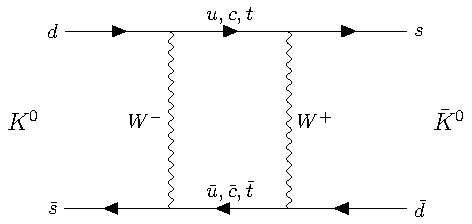
\includegraphics[width=.90\linewidth]{Images/Nu/feynman_kaon_1.pdf}
	\end{subfigure}
	\begin{subfigure}{0.5\textwidth}
		\centering
		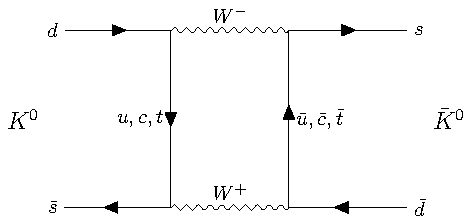
\includegraphics[width=.90\linewidth]{Images//Nu/feynman_kaon_2.pdf}
	\end{subfigure}
	\caption{$K^{0} \leftrightharpoons \bar{K}^{0}$ mixing through $W^{\pm}$ exchange.}
	\label{fig:kaon_oscillations}
\end{figure}

Considering the extended \gls{sm} without any additional sterile neutrino states, the  resulting $3 \times 3$ mixing matrix is unitary. This matrix, often called the Pontecorvo-Maki-Nakagawa-Sakata (\gls{pmns}) matrix \cite{Pontecorvo1957, Maki1962}, relates the set of active neutrinos and the three mass eigenstates as:
\begin{equation}\label{eq:nu_flavour_basis}
\ket{\nu_{\alpha}} = \sum_{i=1}^{3} U^{*}_{\alpha i} \ket{\nu_{i}},
\end{equation}
where the Greek index $\alpha$ denotes the flavour $\{e,\mu,\tau\}$ and the Latin index $i$ the mass state $\{1,2,3\}$. This leptonic mixing matrix may be parametrized in terms of 6 parameters, 3 of which are mixing angles $\theta_{12}$, $\theta_{13}$ and $\theta_{23}$, one \gls{cp}-violating phase $\delta_{CP}$, and 2 Majorana phases $\alpha$ and $\beta$:
\begin{equation}\label{eq:pmns_matrix}
	U = \begin{pmatrix}1&0&0\\0&c_{23}&s_{23}\\0&-s_{23}&c_{23}\end{pmatrix} \begin{pmatrix}c_{13}&0&s_{13} \mathrm{e}^{-i\delta_{CP}}\\0&1&0\\-s_{13} \mathrm{e}^{i\delta_{CP}}&0&c_{13}\end{pmatrix} \begin{pmatrix}c_{12}&s_{12}&0\\-s_{12}&c_{12}&0\\0&0&1\end{pmatrix} \begin{pmatrix}1&0&0\\0&\mathrm{e}^{i\alpha}&0\\0&0&\mathrm{e}^{i\beta}\end{pmatrix},
\end{equation}
where $c_{ij} \equiv \cos \theta_{ij}$ and $s_{ij} \equiv \sin \theta_{ij}$. This matrix is analogous to the Cabibbo-Kobayashi-Maskawa (\gls{ckm}) matrix in the quark sector. If neutrinos are Dirac fermions, we can drop the Majorana phases in the \gls{pmns} matrix, as in this case we can perform the phase redefinitions. In any case, these phases play no role in the neutrino oscillation phenomenology.

In the case that additional sterile neutrinos states are present, the full leptonic mixing matrix would not be unitary in general. For instance, in the see-saw scenario, the $3 \times 3$ submatrix for the three light Majorana neutrinos is not unitary. However, the deviations from unitarity are of the order $\mathcal{O}(M_{D}/M_{N})$, and therefore expected to be negligible.

\subsection{Oscillations in vacuum}

Consider the case where a neutrino of flavour $\alpha$ is produced at $t=0$, and then it propagates through vacuum. Such a state will evolve in time according to the relation \cite{Giganti2017}:
\begin{equation}
\ket{\nu_{\alpha}(\vec{x}, t)} = \sum_{i=1}^{3} U^{*}_{\alpha i} \mathrm{e}^{-i(E_{i}t-\vec{p}_{i}\cdot\vec{x})} \ket{\nu_{i}(\vec{x}=\vec{0},t=0)},
\end{equation}
in the plane wave approximation, as the mass eigenstates are also eigenstates of the free Hamiltonian.
\begin{comment}
Now, if we express the mass eigenstates as a superposition of flavour eigenstates, the last expression can be rewritten as:
\begin{equation}\label{eq:nu_evolution}
\ket{\nu_{\alpha}(t)} = \sum_{\beta} \sum_{i=1}^{3} U_{\beta i} \mathrm{e}^{-iE_{i}t} U^{*}_{\alpha i} \ket{\nu_{\beta}}.
\end{equation}
\end{comment}

This way, the probability for the neutrino to transition from flavour $\alpha$ to flavour $\beta$ will be given by:
\begin{equation}
\begin{split}
	P(\nu_{\alpha} \rightarrow \nu_{\beta}) = \left|\braket{\nu_{\beta}}{\nu_{\alpha}(\vec{x}, t)}\right|^{2} &= \left|\sum_{i=1}^{3} \sum_{j=1}^{3} U^{*}_{\alpha i} U_{\beta j} \mathrm{e}^{-i(E_{i}t-\vec{p}_{i}\cdot\vec{x})} \braket{\nu_{j}}{\nu_{i}}\right|^{2}\\
	&= \left|\sum_{i=1}^{3} U^{*}_{\alpha i} U_{\beta i} \mathrm{e}^{-i(E_{i}t-\vec{p}_{i}\cdot\vec{x})}\right|^{2},
\end{split}
\end{equation}
where we have used the orthogonality relation $\braket{\nu_{i}}{\nu_{j}} = \delta_{ij}$. A usual approximation to take at this point is to consider ultra-relativistic neutrinos, i.e. $p_{i} \simeq E$, so we can write the dispersion relations as:
\begin{equation}
E_{i} = \sqrt{p_{i}^{2} + m_{i}^{2}} \approx E + \frac{m_{i}^{2}}{2 E}.
\end{equation}

In the end, assuming $t \propto L$ where $L$ is the distance between the production and the detection points, the probability for the $\nu_{\alpha} \rightarrow \nu_{\beta}$ transition becomes:
\begin{equation}
\begin{split}
P(\nu_{\alpha} \rightarrow \nu_{\beta}) &= \sum_{i,j} U^{*}_{\alpha i} U_{\beta i} U_{\alpha j} U^{*}_{\beta j} \mathrm{e}^{-i\frac{\Delta m^{2}_{ij}}{2E}L}\\
&=\delta_{\alpha\beta} - 4 \sum_{i<j} \mathfrak{Re}\left[U^{*}_{\alpha i} U_{\beta i} U_{\alpha j} U^{*}_{\beta j}\right] \sin^{2}\left(\frac{\Delta m^{2}_{ij}}{4E}L\right)\\
&\phantom{=}+ 2  \sum_{i<j} \mathfrak{Im}\left[U^{*}_{\alpha i} U_{\beta i} U_{\alpha j} U^{*}_{\beta j}\right] \sin\left(\frac{\Delta m^{2}_{ij}}{2E}L\right),
\end{split}
\end{equation}
where $\Delta m^{2}_{ij}$ is the difference of the squared masses of the $j$th and $i$th neutrino mass eigenstates. A usual way to write the phase responsible for the oscillations is:
\begin{equation}\label{eq:oscillation_term}
\Delta_{ij} \equiv \frac{\Delta m^{2}_{ij}}{4E}L \simeq 1.27 \frac{\Delta m^{2}_{ij}}{(\mathrm{eV}^{2})} \frac{L}{(\mathrm{km})} \frac{(\mathrm{GeV})}{E}.
\end{equation}

Notice that, in the case of antineutrinos, the only difference would be the sign of the last term in the oscillation probability. As the process $\bar{\nu}_{\alpha} \rightarrow \bar{\nu}_{\beta}$ is the \gls{cp}-mirror image of $\nu_{\alpha} \rightarrow \nu_{\beta}$, the differences between their oscillation probabilities would be a measure of \gls{cp} symmetry violation:
\begin{equation}\label{eq:cp_asymmetry}
\begin{split}
A^{\alpha\beta}_{CP}&=P(\nu_{\alpha} \rightarrow \nu_{\beta})-P(\bar{\nu}_{\alpha} \rightarrow \bar{\nu}_{\beta})\\
&=4  \sum_{i<j} \mathfrak{Im}\left[U^{*}_{\alpha i} U_{\beta i} U_{\alpha j} U^{*}_{\beta j}\right] \sin 2\Delta_{ij}.
\end{split}
\end{equation}

Assuming that \gls{cpt} invariance holds, then the following relation must be true:
\begin{equation}
	P(\nu_{\alpha} \rightarrow \nu_{\beta}) = P(\bar{\nu}_{\beta} \rightarrow \bar{\nu}_{\alpha}),
\end{equation}
as these two process are related by the \gls{cpt} symmetry. From the definition of probability, we also must have:
\begin{equation}
	\sum_{\beta} P(\nu_{\alpha} \rightarrow \nu_{\beta}) = \sum_{\beta} P(\bar{\nu}_{\alpha} \rightarrow \bar{\nu}_{\beta}) = 1,
\end{equation}
where the sum includes all flavours (also $\alpha$). From these two constraints, one can prove that:
\begin{equation}
	A^{\alpha\beta}_{CP} = - A^{\beta\alpha}_{CP},
\end{equation}
and in particular:
\begin{equation}
	A^{\alpha\alpha}_{CP} = 0.
\end{equation}

A direct consequence of this last relation is that there are no observable \gls{cp}-violating effects in the so-called disappearance experiments. One needs to perform appearance experiments, where the flavour detected is different from the original flavour, in order to measure the \gls{cp} asymmetry. Neutrino experiments often report the amount of \gls{cp}-violation through the Jarlskog invariant \cite{Jarlskog1985}. In terms of the parametrisation typically used to write the \gls{pmns} matrix, it is given by:
\begin{equation}
	J = \frac{1}{8} \mathrm{cos}~\theta_{13}~\mathrm{sin}~2\theta_{12}~\mathrm{sin}~2\theta_{13}~\mathrm{sin}~2\theta_{23}~\mathrm{sin}~\delta_{CP}.
\end{equation}
The Jarlskog invariant can be used to compare the amount of \gls{cp}-violation in the lepton and the quark sectors, where $J=3.12^{+0.13}_{-0.12} \times 10^{-5}$ in the latter \cite{ParticleDataGroup2024}.

\subsection{Oscillations in matter}

When neutrinos propagate through matter, their oscillation can be affected mainly in two ways. First, neutrinos can inelastically scatter with nuclei, thus destroying the coherent propagation of their quantum state. Nevertheless, in most cases this effect is negligible (even in very dense mediums like the core of the Sun). Second, neutrinos can also experience coherent or forward scatterings, that can affect their oscillation but not lose the coherent propagation of the state.

The first model to account for neutrino oscillations in matter was proposed by S. Mikheev, A. Smirnov and L. Wolfenstein (\gls{msw}) \cite{Wolfenstein1977,Mikheev1986}. It relies on the fact that, as the only charged lepton present in ordinary matter is the electron, electron neutrinos can undergo both charged and neutral-current interactions with matter, whereas for muon and tau neutrinos just neutral current processes are possible.

An illustrative way to introduce the \gls{msw} mechanism is by considering the two flavour case. It can be shown that the evolution of the two flavour eigenstates in vacuum is given by the following time-dependent Schrödinger equation:
\begin{equation}
	i \frac{\mathrm{d}}{\mathrm{d}t} \begin{pmatrix}\nu_{e}\\\nu_{\mu}\end{pmatrix} = H_{V} \begin{pmatrix}\nu_{e}\\\nu_{\mu}\end{pmatrix},
\end{equation}
with a vacuum Hamiltonian given by:
\begin{comment}
\begin{equation}
	H_{V} = \frac{m_{1}^{2}+m_{2}^{2}}{4E} \begin{pmatrix}1&0\\0&1\end{pmatrix}+\frac{\Delta m^{2}}{4E} \begin{pmatrix}-\mathrm{cos}~2\theta&\mathrm{sin}~2\theta\\\mathrm{sin}~2\theta&\mathrm{cos}~2\theta\end{pmatrix},
\end{equation}
\end{comment}
\begin{equation}
	H_{V} = \frac{\Delta m^{2}}{4E} \begin{pmatrix}-\mathrm{cos}~2\theta&\mathrm{sin}~2\theta\\\mathrm{sin}~2\theta&\mathrm{cos}~2\theta\end{pmatrix},
\end{equation}
where $\Delta m^{2}$ is the mass splitting between the two neutrino states and $\theta$ the only mixing angle. For simplicity, I omit the terms of the Hamiltonian that are proportional to the identity, as they do not affect the oscillation phenomenology.

The \gls{nc} contribution to the matter potential is identical for all the flavours, and has the form:
\begin{equation}
	V_{\mathrm{NC}} = -\frac{G_{F}}{\sqrt{2}} N_{n}(x),
\end{equation}
where $G_{F}$ is the Fermi constant and $N_{n}(x)$ the local neutron density. Because it is common to all flavours, I do not take it into account in the effective Hamiltonian, as it would appear as a term proportional to the identity. The \gls{cc} component only affects the electron neutrino (and antineutrino). It can be written as:
\begin{equation}
	V_{\mathrm{CC}} = \pm \sqrt{2} G_{F} N_{e}(x),
\end{equation}
with $N_{e}(x)$ being the local electron density in the material. In the end, the effective Hamiltonian which describes the propagation of the flavour eigenstates in matter only contains an extra $\nu_{e}-\nu_{e}$ element:
\begin{equation}
	H_{M} = H_{V} + \begin{pmatrix}V_{\mathrm{CC}}&0\\0&0\end{pmatrix}.
\end{equation}

The solution to the Schrödinger equation greatly simplifies if one considers the case of a constant matter density. In that case, the effective Hamiltonian can be diagonalised, obtaining the effective neutrino mass eigenstates in matter. It can be re-written in the same form as the vacuum Hamiltonian:
\begin{equation}
	H_{M} = \frac{\Delta m_{m}^{2}}{4E} \begin{pmatrix}-\mathrm{cos}~2\theta_{m}&\mathrm{sin}~2\theta_{m}\\\mathrm{sin}~2\theta_{m}&\mathrm{cos}~2\theta_{m}\end{pmatrix},
\end{equation}
where the effective mass splitting and the effective mixing angle are given by:
\begin{equation}
	\begin{split}
		\Delta m_{m}^{2} = \lambda \Delta m^{2},\\
		\mathrm{sin}~2\theta_{m} = \frac{\mathrm{sin}~2\theta}{\lambda},
	\end{split}
\end{equation}
with:
\begin{equation}
	\begin{split}
		\lambda &= \sqrt{(\mathrm{cos}~2\theta - A)^{2} + \mathrm{sin}^{2}~2\theta},\\
		A &= \pm \frac{2\sqrt{2}G_{F}N_{e}E}{\Delta m^{2}}.
	\end{split}
\end{equation}

In terms of the effective matter oscillation parameters, the transition probability $\nu_{e} \rightarrow \nu_{\mu}$ (in the two flavour approximation) reads:
\begin{equation}
	P(\nu_{e} \rightarrow \nu_{\mu}) = \mathrm{sin}^{2}~2\theta_{m} ~ \mathrm{sin}^{2}\left(\frac{\Delta m_{m}^{2}}{2E}L\right)
\end{equation}
From this last equation one can see that, when $\mathrm{cos}~2\theta = A > 0$ the oscillations are greatly enhanced. This effect is known as the \gls{msw} resonance. For the neutrinos, this resonant condition is only satisfied if $\Delta m^{2}>0$ (the opposite is true for antineutrinos). This can be exploited by long-baseline experiments, which can gain sensitivity to the neutrino mass hierarchy through matter effects.

\subsection{Current status of neutrino oscillations}

A wide range of neutrino experiments provide experimental input to the neutrino oscillation framework, both using natural or human-made neutrino sources. The results from one of the neutrino global fit analyses, shown in Tab. \ref{tab:neutrino_global_fit} \footnote{These are the updated results reported during M. T\'{o}rtola's talk at Neutrino 2024 (see this \href{https://agenda.infn.it/event/37867/contributions/233956/attachments/121839/178002/MTortola-Neutrino2024.pdf}{link}).}, summarise well our current understanding of the different oscillation parameters.

\textbf{Solar neutrino experiments} detect neutrinos produced in thermonuclear reactions inside the Sun, mainly from the so-called $\mathrm{p}-\mathrm{p}$ chain and the CNO cycle. These neutrinos have a typical energy in the range from $0.1$ to $20 \ \mathrm{MeV}$. These experiments (Homestake \cite{Homestake1998}, \gls{gallex} \cite{GALLEX2010}, \gls{sage} \cite{SAGE2009}, Borexino \cite{Borexino2011}, \gls{sk} \cite{Super-Kamiokande2005} and \gls{sno} \cite{SNO2011}) provide the best sensitivities to $\theta_{12}$ and $\Delta m^{2}_{21}$.

\textbf{Atmospheric neutrino experiments} detect the neutrino flux produced when cosmic rays scatter with particles in Earth's atmosphere. These collisions generate particle showers that eventually produce electron and muon neutrinos (and antineutrinos). Their energies range from few $\mathrm{MeV}$ to about $10^{9} \ \mathrm{GeV}$. Experiments like \gls{sk} \cite{Super-Kamiokande2017} and IceCube \cite{IceCube2017} use atmospheric neutrinos to measure oscillations, and are specially sensitive to $\theta_{23}$ and $\Delta m^{2}_{32}$.

\textbf{Reactor neutrino experiments} look for the $\bar{\nu}_{e}$ spectrum produced by nuclear reactors, with energies in the $\mathrm{MeV}$ scale. Depending on the distance to the source, long-baseline experiments like \gls{kamland} \cite{KamLAND2013} are sensitive to the solar mass splitting $\Delta m^{2}_{21}$, whereas much shorter baseline experiments such as \gls{reno} \cite{RENO2018} or DayaBay \cite{DayaBay2018} measure $\theta_{13}$ and $\Delta m^{2}_{31}$.

\textbf{Accelerator experiments} measure neutrino interactions from beams generated by particle accelerators. Mesons are produced when the protons from the accelerator collide into a target. These are then focused into a beam, with some of them decaying into muon neutrinos while the rest are removed from the beam by an absorber. Depending on the configuration one can obtain a beam made of mostly neutrinos or antineutrinos. The typical energies of these neutrinos are in the $\mathrm{GeV}$ range. Experiments such as \gls{nova} \cite{NOvA2023}, \gls{t2k} \cite{T2K2023}, \gls{minos} \cite{MINOS2014}, OPERA \cite{OPERA2018} and \gls{k2k} \cite{K2K2006} (and in the future \gls{dune} \cite{DUNE2020}) are primarily sensitive to $\theta_{13}$, $\theta_{23}$ and $\Delta m^{2}_{32}$. Also, in the coming years \gls{dune} \cite{DUNE2020} and Hyper-Kamiokande (\gls{hk}) \cite{Hyper-Kamiokande2019} will be sensitive to $\delta_{CP}$.

\begin{table}
	\caption[Summary of neutrino oscillation parameters determined in the Neutrino Global Fit of 2020.]{Summary of neutrino oscillation parameters determined in the Neutrino Global Fit of 2020 \cite{deSalas2020}.}
	\begin{center}
		\begin{small}
			\begin{tabular}{c|c|c}
				Parameter                                               & Best fit $\pm ~ 1\sigma$ & $3 \sigma$ range   \\[1mm] \hline \rule{0pt}{1.1\normalbaselineskip}
				$\Delta m^{2}_{21}~[\mathrm{eV}^{2} \times 10^{-5}]$                   & $7.55^{+0.22}_{-0.20}$ & $6.98-8.19$\\[3mm]
				$\left|\Delta m^{2}_{31}\right|~[\mathrm{eV}^{2}\times 10^{-3}]$ (\gls{no}) & $2.51^{+0.02}_{-0.03}$    & $2.43-2.58$\\[2mm]
				$\left|\Delta m^{2}_{31}\right|~[\mathrm{eV}^{2}\times 10^{-3}]$ (\gls{io}) & $2.41^{+0.03}_{-0.02}$ & $2.34-2.49$    \\[3mm]
				$\sin^{2} \theta_{12} / 10^{-1}$ & $3.04 \pm 0.16$ & $2.57-3.55$ \\[3mm]
				$\sin^{2} \theta_{23} / 10^{-1}$ (\gls{no}) & $5.64^{+0.15}_{-0.21}$ & $4.23-6.04$ \\[2mm]
				$\sin^{2} \theta_{23} / 10^{-1}$ (\gls{io}) & $5.64^{+0.15}_{-0.18}$ & $4.27-6.03$ \\[3mm]
				$\sin^{2} \theta_{13} / 10^{-2}$ (\gls{no}) & $2.20^{+0.05}_{-0.06}$ & $2.03-2.38$ \\[2mm]
				$\sin^{2} \theta_{13} / 10^{-2}$ (\gls{io}) & $2.20^{+0.07}_{-0.04}$ & $2.04-2.38$ \\[3mm]
				$\delta_{CP} / \pi$ (\gls{no}) & $1.12^{+0.16}_{-0.12}$ & $0.76-2.00$ \\[2mm]
				$\delta_{CP} / \pi$ (\gls{io}) & $1.50^{+0.13}_{-0.14}$ & $1.11-1.87$
			\end{tabular}
		\end{small}
	\end{center}
	\label{tab:neutrino_global_fit}
\end{table}

\section{Open questions in the neutrino sector}\label{sec:nu_open_questions}

A crucial question that remains open these days, and is of vital importance for the oscillation phenomenology, is whether the mass eigenstate $\nu_{3}$ is the heaviest (what we call normal ordering) or the lightest (referred to as inverted ordering) of the mass states. In other words, this means that we do not know the sign of $\Delta m^{2}_{32}$, so we can either have $m_{1}<m_{2}<m_{3}$ (\gls{no}) or $m_{3}<m_{1}<m_{2}$ (\gls{io}).

Also relevant to the neutrino oscillations, there is the problem regarding the $\theta_{23}$ octant. Previous experimental results were compatible with its value being close to maximal, $\theta_{23} \sim 45^{\circ}$ \cite{T2K2015,NOvA2016}. However, global data fits indicate a deviation from the maximal mixing, giving rise to two degenerate solutions, one in the lower octant $\theta_{23} < 45^{\circ}$ and another in the higher octant $\theta_{23} > 45^{\circ}$ (see e.g. Ref. \cite{deSalas2020}).

\begin{comment}
	Another big puzzle is related to the value of $\delta_{CP}$. Nowadays it is poorly constrained, with all values between $\pi$ and $2\pi$ being consistent with data. A prospective measurement different from $\delta_{CP}=0,\pm\pi$ will be a sign of \gls{cp}-violation in the leptonic sector, and thus contribute along with the one measured in the quark sector to the total amount of \gls{cp}-violation. Although it is true that these two contributions by themselves are not enough to explain the matter anti-matter asymmetry in our universe, the amount of \gls{cp}-violation in the leptonic sector can be key to explain such imbalance.
\end{comment}

Another big puzzle is related to the value of $\delta_{CP}$. Nowadays it is poorly constrained, with all values between $\pi$ and $2\pi$ being consistent with data. A prospective measurement different from $\delta_{CP}=0,\pm\pi$ will be a sign of \gls{cp}-violation in the leptonic sector, and thus contribute along with that measured in the quark sector to the total amount of \gls{cp}-violation. The amount of \gls{cp}-violation in the leptonic sector can be key to explain the matter anti-matter asymmetry in our universe, through the process referred to as leptogenesis \cite{Davidson2008}.

These three questions, because of their nature, could be understood thanks to the next generation of oscillation experiments, like \gls{dune}.

Notwithstanding, there are other mysteries that can not be unveiled just by conducting oscillation experiments, as certain quantities do not influence these phenomena. Among these there is the question of the absolute values of the neutrino masses. Depending on the value of the lightest of the neutrino masses we can have different mass spectra, from hierarchical $m_{1} \ll m_{2}<m_{3}$ (\gls{no}) or $m_{3} \ll m_{1}<m_{2}$ (\gls{io}) to quasi-degenerate $m_{1} \simeq m_{2} \simeq m_{3}$.

Other open question concerns the nature of the neutrinos themselves. If neutrinos are Dirac particles then their mass term can be generated through the usual Higgs mechanism by adding right-handed neutrino fields. However, if they are Majorana particles and therefore their own antiparticles, there is no need to add extra fields to have the mass term in the Lagrangian. Experiments like \gls{supernemo} \cite{SuperNEMO2010}, \gls{sno}+ \cite{SNO2015}, and \gls{next} \cite{NEXT2020}, which search for neutrino-less double beta decay, will be able to determine whether neutrinos are Dirac or Majorana particles.

\section{Neutrino interactions}\label{sec:nu_interactions}

% Introduction
The study of neutrino-nucleus interactions is of great importance for long baseline neutrino oscillation experiments. The interaction model provides a mapping between the energy of the incoming neutrino and the final state particles after the interaction. Because in these kinds of experiments neutrinos are obtained as secondary decay products of mesons, typically charged pions and kaons, their energies are not known a priori. Not only that, but the kinematics of the interacting nuclei are also unknown. Therefore, we rely on the neutrino interaction models to provide this relation between the observables in the detector and the true kinematics of the neutrino. Limited understanding of the interaction modelling is expected to be the one of the leading sources of systematic uncertainties in the next generation of long-baseline experiments \cite{Coloma2013,Coloma2013a,Mosel2016}.

\begin{figure}[t]
	\begin{subfigure}{0.5\textwidth}
		\centering
		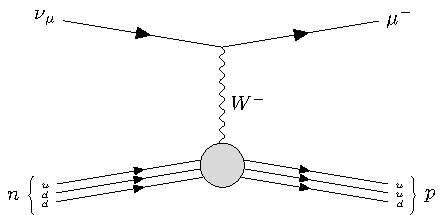
\includegraphics[width=.90\linewidth]{Images/Nu/feynman_ccqel.pdf}
		\caption{Quasi-elastic.}
	\end{subfigure}
	\begin{subfigure}{0.5\textwidth}
		\centering
		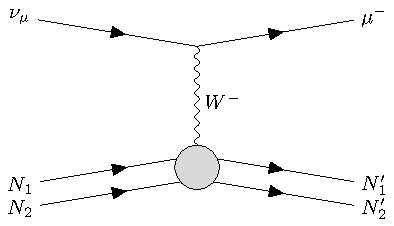
\includegraphics[width=.90\linewidth]{Images//Nu/feynman_ccmec.pdf}
		\caption{$2p2h$.}
	\end{subfigure}
	\begin{subfigure}{0.5\textwidth}
		\centering
		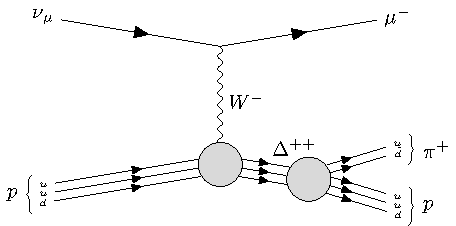
\includegraphics[width=.90\linewidth]{Images//Nu/feynman_ccres_delta++.pdf}
		\caption{\gls{res} ($\Delta^{++} \rightarrow p + \pi^{+}$).}
	\end{subfigure}
	\begin{subfigure}{0.5\textwidth}
		\centering
		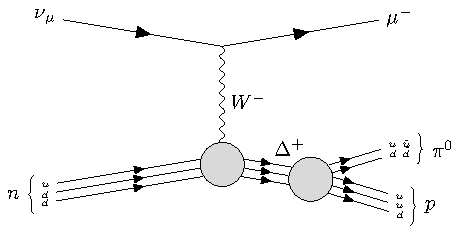
\includegraphics[width=.90\linewidth]{Images//Nu/feynman_ccres_delta+.pdf}
		\caption{\gls{res} ($\Delta^{+} \rightarrow p + \pi^{0}$).}
	\end{subfigure}
	\begin{subfigure}{0.5\textwidth}
		\centering
		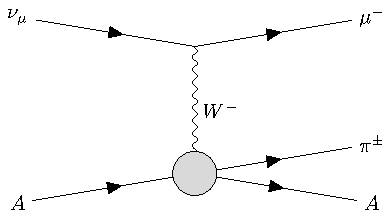
\includegraphics[width=.90\linewidth]{Images//Nu/feynman_cccoh.pdf}
		\caption{Coherent.}
	\end{subfigure}
	\begin{subfigure}{0.5\textwidth}
		\centering
		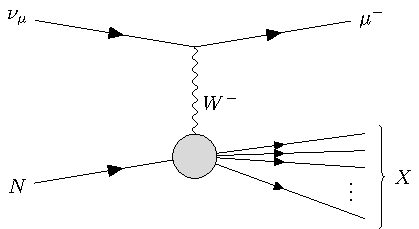
\includegraphics[width=.90\linewidth]{Images//Nu/feynman_ccdis.pdf}
		\caption{Deep inelastic.}
	\end{subfigure}
	\caption{Feynman diagrams of the most relevant \gls{cc} interactions to long-baseline neutrino oscillation experiments.}
	\label{fig:neutrino_cc_interactions}
\end{figure}

% Neutrino-nucleon interactions
\begin{comment}
In the case of neutrino interactions with nuclei, at the energies relevant for long baseline oscillation experiments, around the $\mathrm{GeV}$-scale, the process is dominated by the interaction between the neutrino and a single nucleon within the nuclear medium. Figure \ref{fig:neutrino_cc_interactions} shows examples of the most common neutrino \gls{cc} interactions. In these diagrams, $A$ indicates that the interaction happened with the nucleus as a whole, whereas $N$ denotes a single nucleon.
\end{comment}

In long-baseline neutrino oscillation experiments, the energies relevant for the neutrino interactions with nuclei sit around the $\mathrm{GeV}$-scale. Figure \ref{fig:neutrino_cc_interactions} shows examples of the most common neutrino \gls{cc} interactions in this energy range. In these diagrams, $A$ indicates that the interaction happened with the nucleus as a whole, whereas $N$ denotes a single nucleon.

\begin{figure}[t]
	\centering
	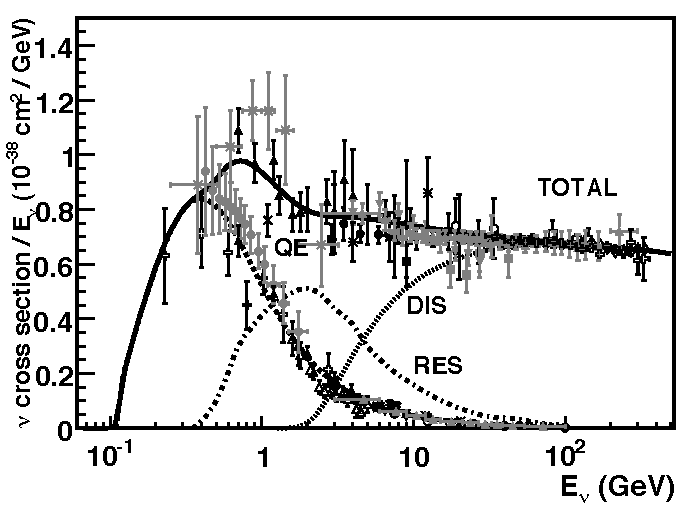
\includegraphics[width=.85\linewidth]{Images/Nu/numu_cc_cross_section.pdf}
	\caption[Total muon neutrino \gls{cc} cross section per nucleon as a function of the neutrino energy.]{Total $\nu_{\mu}$ \gls{cc} cross section per nucleon as a function of the neutrino energy. The contributions from the different channels are shown. Figure taken from Ref. \cite{Formaggio2012}.}
	\label{fig:numu_cc_cross_section}
\end{figure}

At low energies, below $1~\mathrm{GeV}$, quasi-elastic (\gls{qe}) interactions dominate. In a \gls{cc}\gls{qe} interaction a neutrino (antineutrino) interacts with a neutron (proton), converting it into a proton (neutron) which is then ejected from the nucleus together with the resulting charged lepton. Neutrinos can also scatter off bound states of nucleons inside the nucleus. These interactions are typically denoted as $npnh$, as the neutrino interacts with a bound state of $n$ nucleons and leave $n$ holes in the nucleus. Particularly relevant are the $2p2h$ events, as distinguishing them from pure \gls{cc}\gls{qe} events is challenging. The $2p2h$ neutrino interactions are dominated by meson exchange current events (\gls{mec}), where the nucleons are bound by the exchange of a virtual meson.

At energies above $1~\mathrm{GeV}$ the neutrino is able to excite the nucleons into a baryonic resonance, which promptly decays into a nucleon and a pion. These are the so-called resonant (\gls{res}) interactions. Neutrinos also interact with entire nuclei coherently, in the process known as coherent (\gls{coh}) interaction. These kinds of reactions also produce a single pion in the final state. At high neutrino energies, above $5~\mathrm{GeV}$, deep inelastic scattering (\gls{dis}) takes place. In these processes, the neutrino interacts with a single quark within the nucleon, breaking the nucleon and producing a hadronic shower.

Figure \ref{fig:numu_cc_cross_section} shows a compilation of measurements of the total $\nu_{\mu}$ \gls{cc} cross section (see Ref. \cite{Formaggio2012} for the details of the different experimental results). Also shown are the contributions from the different interaction modes. The contribution of the \gls{cc}\gls{coh} interaction is omitted, as it is negligible compared to the others. This shows how the interaction model needs to accurately predict the neutrino-nucleon cross section for the different interaction modes across a broad energy range, to obtain the correct relative contributions.

\begin{figure}[t]
	\centering
	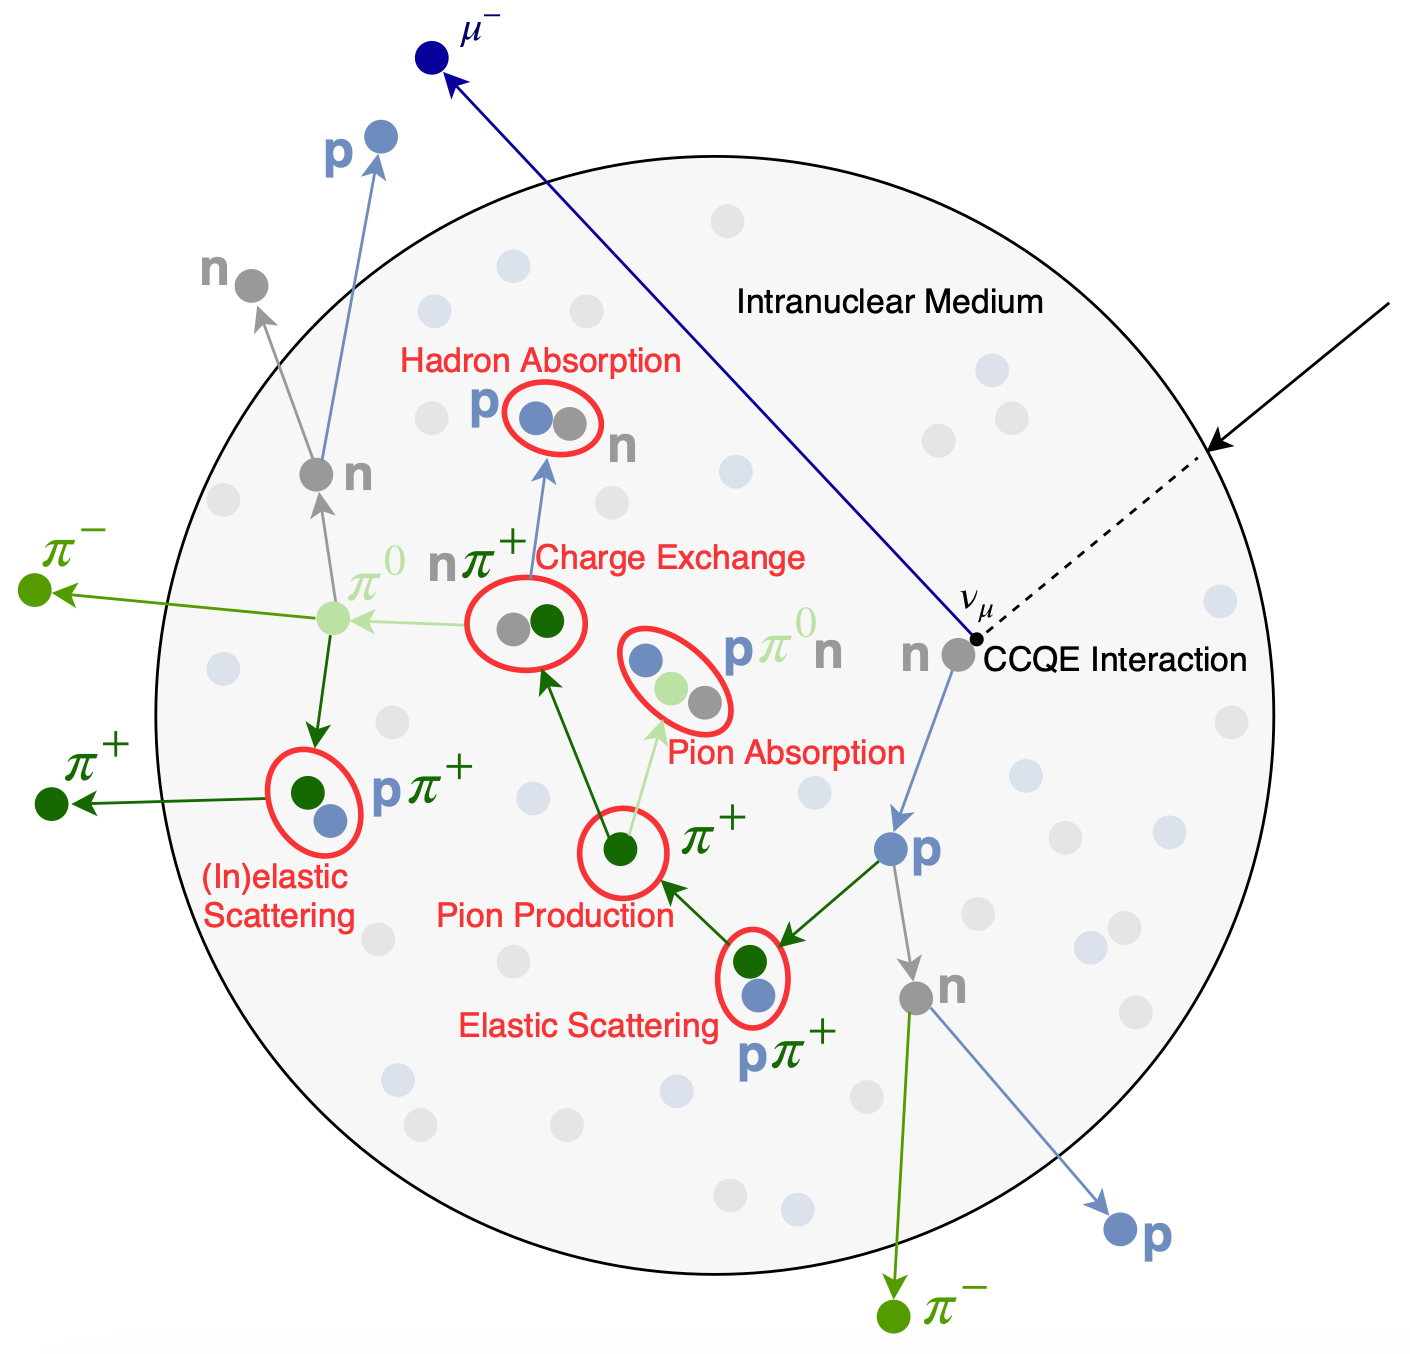
\includegraphics[width=.55\linewidth]{Images/Nu/lars_fsi.png}
	\caption[Schematic representation of a $\nu_{\mu}$ \gls{cc}\gls{qe} interaction with a neutron inside a nucleus.]{Schematic representation of a $\nu_{\mu}$ \gls{cc}\gls{qe} interaction with a neutron inside a nucleus. The reaction produces a muon and a proton, which travel through the nuclear medium. The outgoing proton undergoes various kinds of hadronic \gls{fsi}s on its way out. Figure taken from Ref. \cite{Bathe-Peters2022}.}
	\label{fig:fsi_diagram}
\end{figure}

% Nuclear effects and FSI
Nuclear effects alter the neutrino cross section, as well as the multiplicities of the final state particles. Therefore, the interaction models need to account for the effects introduced by the nuclei. There are several models available to describe the initial state of the nucleus, like the relativistic Fermi gas model \cite{Smith1972}, the local Fermi gas model \cite{Chiang1989}, or spectral functions \cite{Nakamura2002}. The other main effect that interaction models have to deal with are the so-called final state interactions (\gls{fsi}). These are the interactions of the particles produced in the neutrino-nucleon scattering as they travel through the nuclear medium. Typically, the lepton exits the nucleus without interacting. However, hadrons tend to get scattered, absorbed or re-emitted. These effects are usually described by means of intra-nuclear cascade models \cite{Nikolakopoulos2022}. Figure \ref{fig:fsi_diagram} illustrates the effects of \gls{fsi} on the observable particle content in the detector after a $\nu_{\mu}$ \gls{cc}\gls{qe} interaction.

% Experimental status
There exists a rich experimental programme dedicated to the measurement of neutrino cross sections. The list of such experiments in the recent years include Mini\gls{boone} \cite{MiniBooNE2010}, \gls{minerva} \cite{MINERvA2016}, Micro\gls{boone} \cite{MicroBooNE2021} and \gls{sbnd} \cite{McConkey2018}. Additionally, thanks to their near detectors, long-baseline experiments can perform cross section measurements. Some recent examples are \gls{nova} \cite{Nova2021} or \gls{t2k} \cite{T2K2019}. Future oscillation experiments will greatly benefit from these measurements, as the measurement of the oscillation parameters depends on the cross-section modelling. However, there are alternative data-driven approaches to extract the oscillation probabilities without relying on a neutrino interaction model, which are planned to be explored in the next generation of experiments \cite{Scott2015,Hasnip2023}. The importance of the near detector in long-baseline oscillation experiments, and in particular in the context of \gls{dune}, will be discussed further in the next Chapters.